\subsection{Model}

\begin{frame}[fragile]{Problem presentation}

\begin{columns}
\begin{column}{0.5\textwidth}
\only<2>{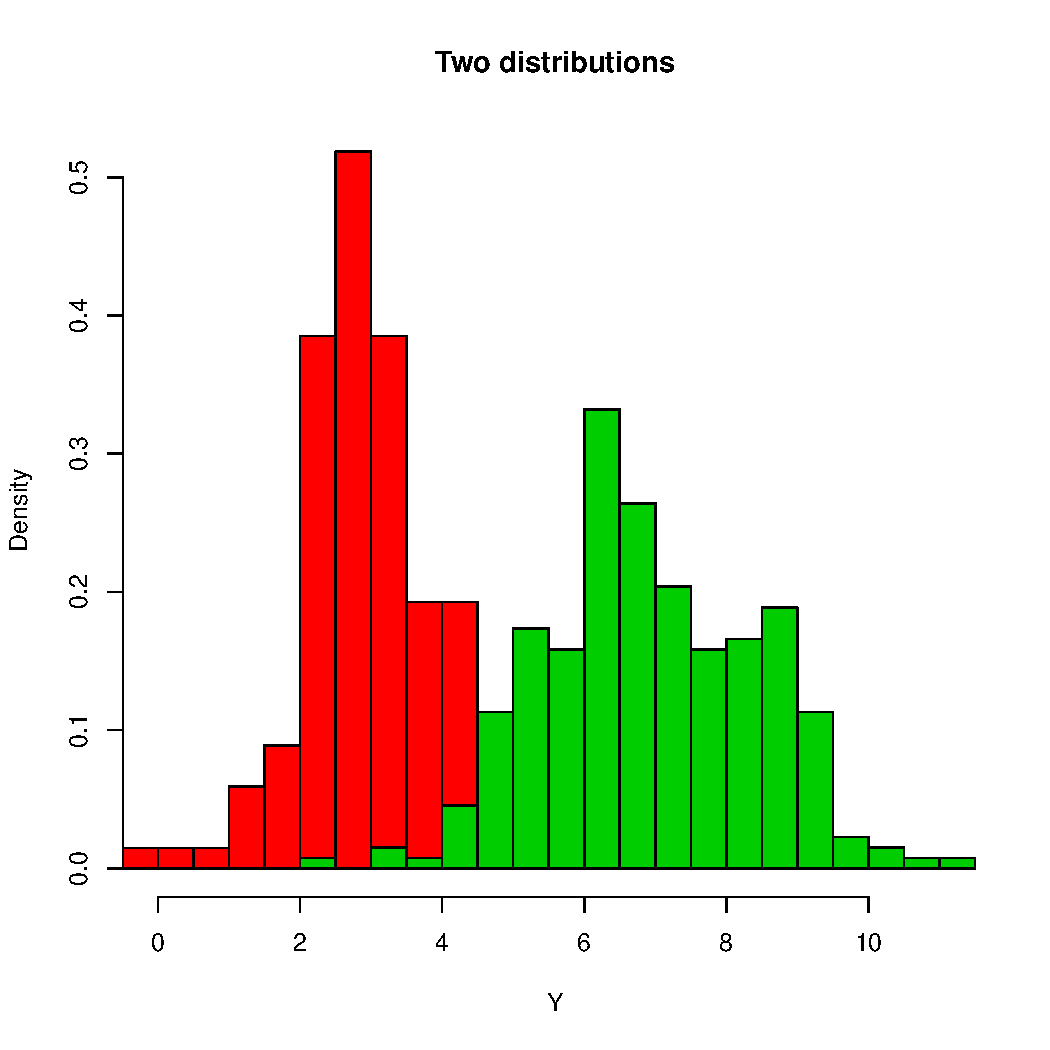
\includegraphics[scale=0.3]{mixCode1-5.pdf}}
\only<3->{\paragraph{Basic idea :}\\
 "Expert" threshold $s$ \\  
 $$ State_i=1 \quad \mbox{if} Y_i<s$$
 $$ State_i=2 \quad \mbox{if} Y_i\geq  s $$
}
\only<5->{\paragraph{Improvement:}\\
 \textcolor{blue}{Estimating} the threshold s and  reconstruction of the hidden state (colour)\\
 Compute the \textcolor{blue}{probability to belong} to State 1 or 2.\\
}
 \only<6->{
 \bigskip
   \centering{$\Longrightarrow$ \textcolor{red}{Mixture Model}}
 }
 \end{column}
 \begin{column}{0.4\textwidth}

 \only<1>{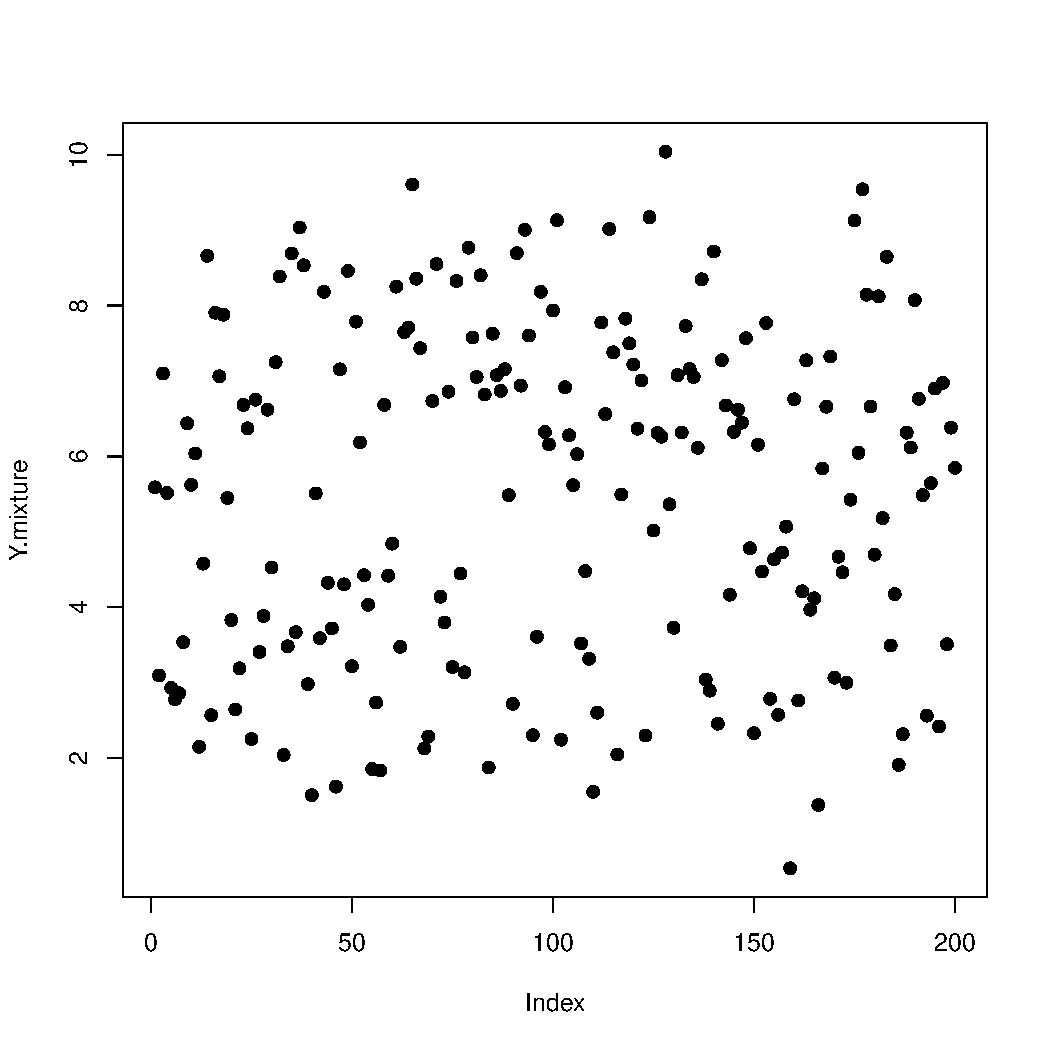
\includegraphics[scale=0.3]{mixCode1-1.pdf}}
 \only<2>{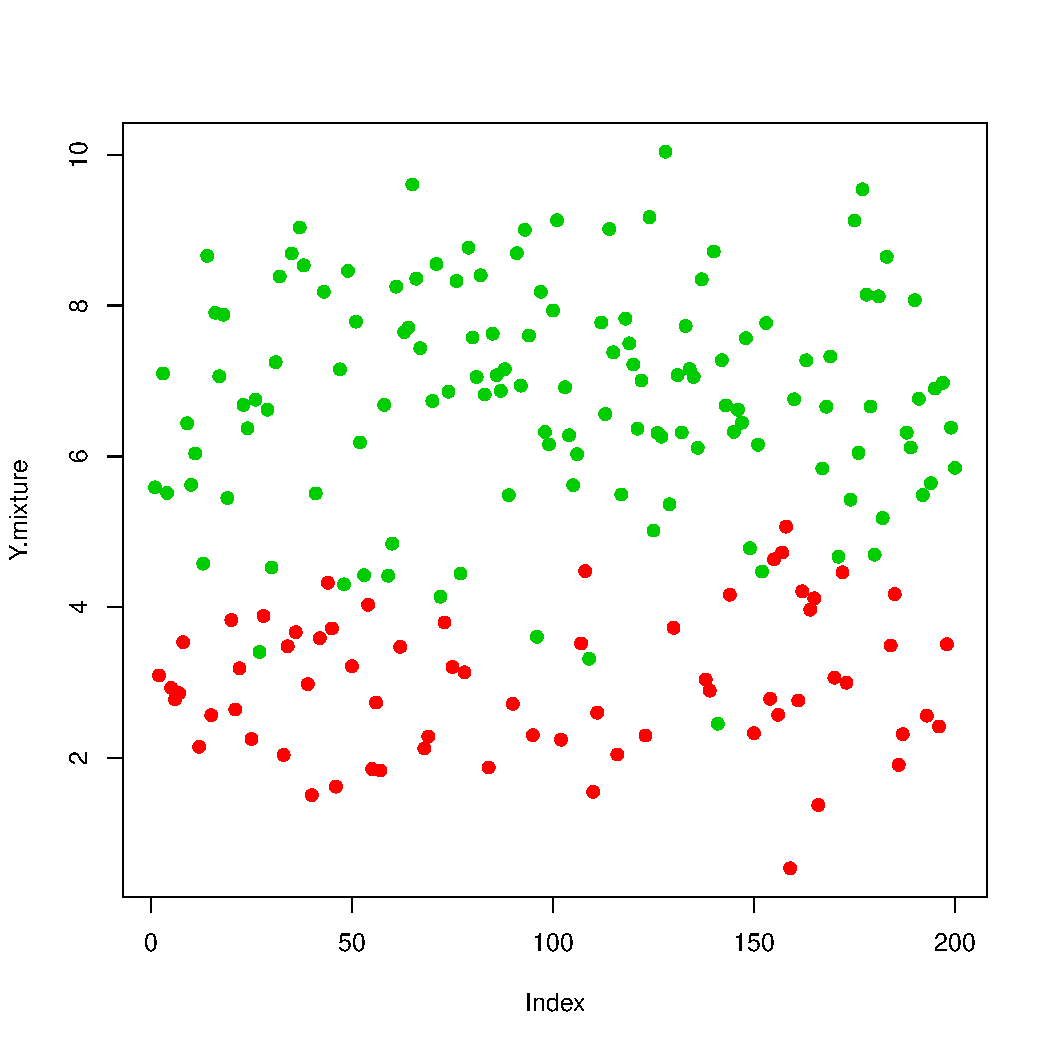
\includegraphics[scale=0.3]{mixCode1-2.pdf}}
 \only<3>{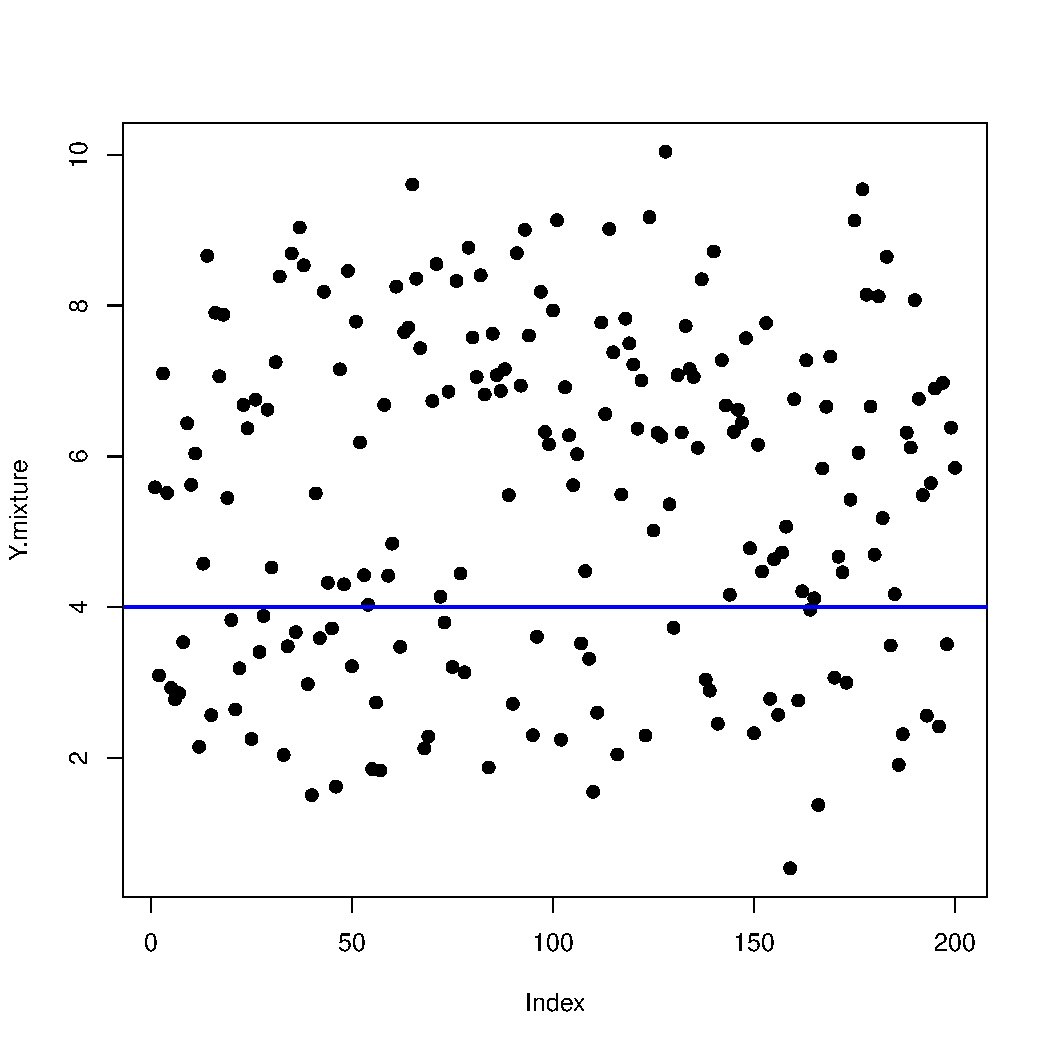
\includegraphics[scale=0.3]{mixCode1-3.pdf}}
 \only<4->{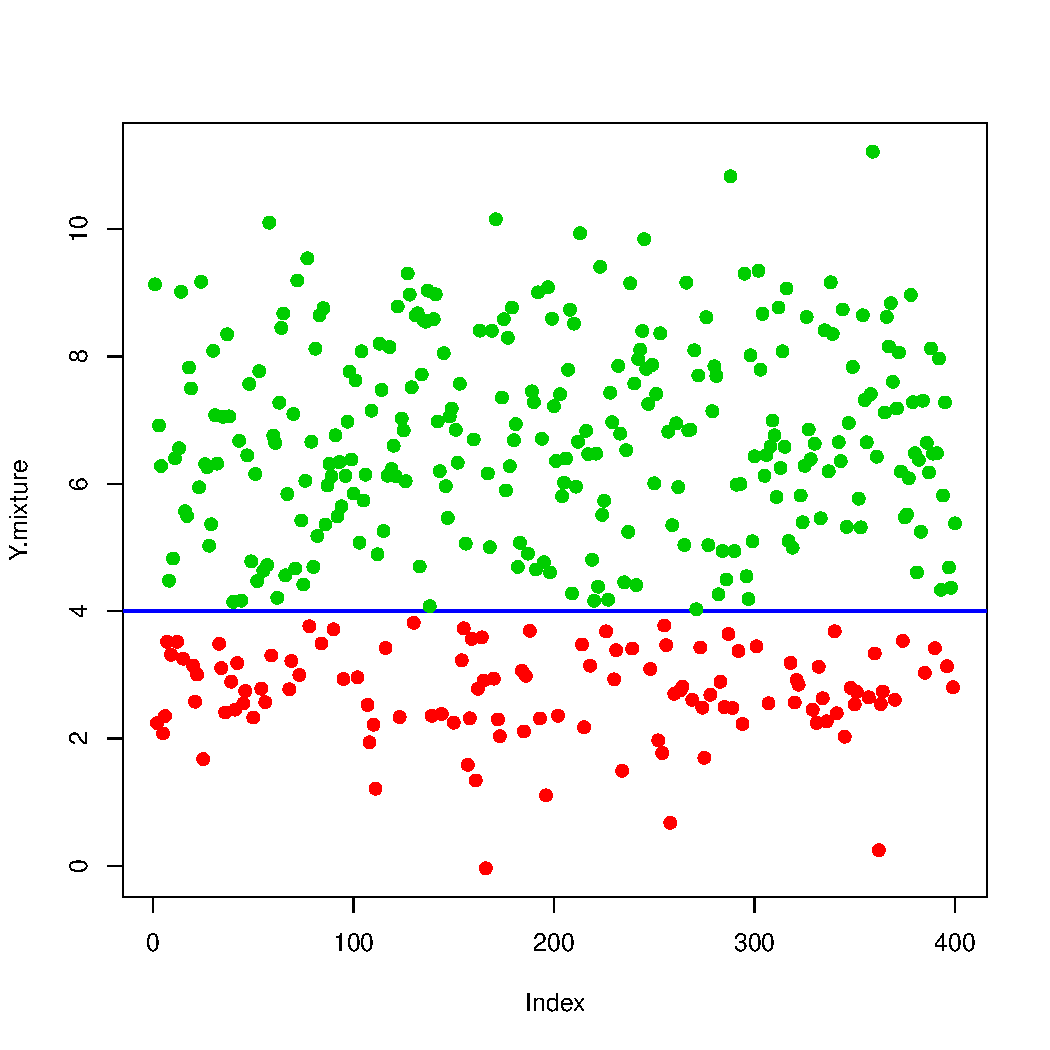
\includegraphics[scale=0.3]{mixCode1-4.pdf}}
\end{column}
\end{columns}
\end{frame}

%%-----------------------------------------------------------------%%
%%-----------------------------------------------------------------%%

\begin{frame}[fragile]{Proposed model}
\paragraph{Model}
For a given number of states $K$, 
\begin{itemize}
\item
 \blue{Modelling $Z$}: $\pi_k=\P(Z_i=k), \quad k=1,\ldots, K, \quad \sum_k \pi_k=1$\par
 $Z_i \overset{i.i.d}{\sim} \Mcal(1, \pibf), \quad P(Z_{ik}=1)=\pi_k$
 \item \blue{Modelling $Y$}: The $Y_i's$ are assumed to be independent  conditionnaly to $\Zbf$ : $(Y_i\vert Z_i = k) \overset{i.i.d}{\sim} f_{\theta_k}().$
\end{itemize}
 \onslide<2->{\centering{\blue{Model parameters are $\pibf$ and $\thetabf$}}\par}
 \onslide<3->{\centering{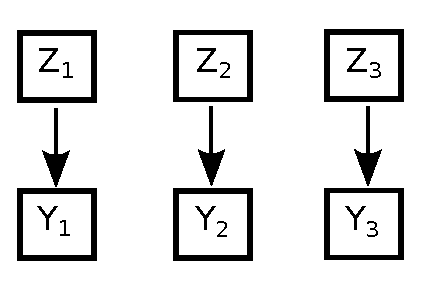
\includegraphics[scale=0.4]{Dag2.pdf}}}
\end{frame}

\begin{frame}[fragile]{Proposed model}
\paragraph{Model}
For a given number of states $K$, 
\begin{itemize}
\item
 \blue{Modelling $Z$}: $\pi_k=\P(Z_i=k), \quad k=1,\ldots, K, \quad \sum_k \pi_k=1$\par
 $Z_i \overset{i.i.d}{\sim} \Mcal(1, \pibf)$
 \item \blue{Modelling $Y$}: The $Y_i's$ are assumed to be independent  conditionnaly to $\Zbf$ : $(Y_i\vert Z_i = k) \overset{i.i.d}{\sim} f_{\theta_k}().$
\end{itemize}
\begin{columns}
  \begin{column}{0.45\textwidth}
\begin{knitrout}
\definecolor{shadecolor}{rgb}{0.969, 0.969, 0.969}\color{fgcolor}\begin{kframe}
\begin{alltt}
\hlstd{K} \hlkwb{<-} \hlnum{2}\hlstd{; N} \hlkwb{<-} \hlnum{200}\hlstd{; mu} \hlkwb{<-} \hlkwd{c}\hlstd{(}\hlnum{3}\hlstd{,} \hlnum{6}\hlstd{); sigma} \hlkwb{<-} \hlkwd{c}\hlstd{(}\hlnum{1}\hlstd{,}\hlnum{1.5}\hlstd{)}
\hlstd{Z} \hlkwb{<-} \hlkwd{sample}\hlstd{(}\hlnum{1}\hlopt{:}\hlnum{2}\hlstd{,} \hlkwc{size} \hlstd{= N,} \hlkwc{replace}\hlstd{=T,} \hlkwc{prob}\hlstd{=}\hlkwd{c}\hlstd{(}\hlnum{0.3}\hlstd{,} \hlnum{0.7}\hlstd{))}
\hlkwd{plot}\hlstd{(Z,} \hlkwc{col}\hlstd{=Z}\hlopt{+}\hlnum{1}\hlstd{,} \hlkwc{pch}\hlstd{=}\hlnum{15}\hlstd{)}
\hlstd{Y.mixture} \hlkwb{<-} \hlkwd{rnorm}\hlstd{(N,} \hlkwc{mean}\hlstd{=mu[Z],} \hlkwc{sd}\hlstd{=sigma[Z])}
\hlkwd{plot}\hlstd{(Y.mixture,} \hlkwc{col}\hlstd{=Z}\hlopt{+}\hlnum{1}\hlstd{,} \hlkwc{pch}\hlstd{=}\hlnum{19}\hlstd{)}
\end{alltt}
\end{kframe}
\end{knitrout}
 \end{column}
  \begin{column}{0.45\textwidth}
    \only<3>{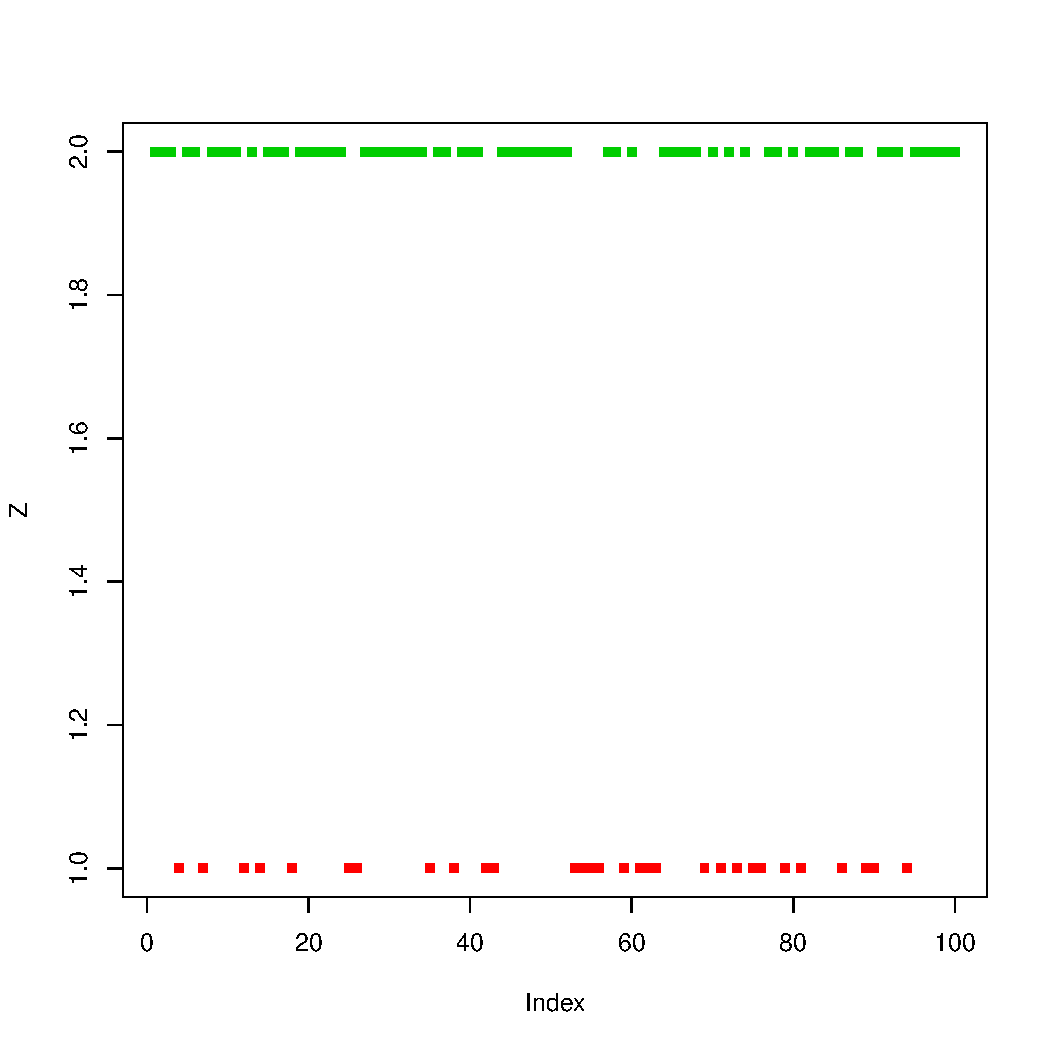
\includegraphics[height=3cm, width=6cm]{mixCode2-1.pdf}}
    \only<4->{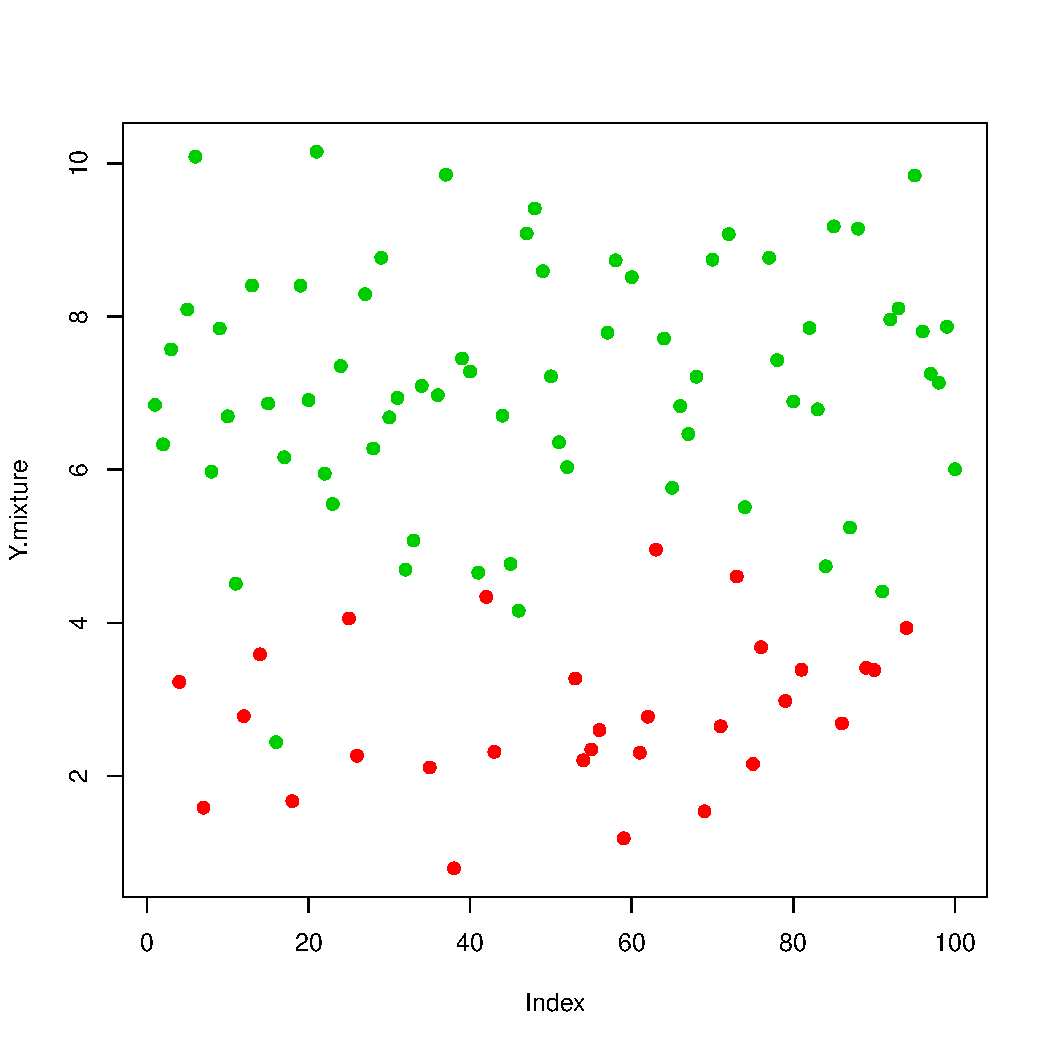
\includegraphics[scale=0.25]{mixCode2-2.pdf}}
  \end{column}
  \end{columns}
\end{frame}

\begin{frame}[fragile]{Model Properties}
\begin{itemize}
\item Couples $\{(Y_i, Z_i)\}$ are i.i.d.
\item \blue{Label switching}:\\ the model is invariant for any permutation of the labels $\{1,
  \dots, K\}$ $\Rightarrow$ the mixture model has \emphase{$K!$
    equivalent definitions}.
\item\blue{Distribution of a $Y_i$:}\\
$$P(Y_i)=\sum_{k=1}^K P(Y_i, Z_i=k)=\textcolor{blue}{P(Z_i=k)} \textcolor{magenta}{P(Y_i | Z_i=k)} $$
\item\blue{Distribution of $\Ybf$:}\\
{\small
\begin{eqnarray*}
P(\Ybf ; \thetabf, \pibf)= \prod_{i=1}^n \sum_{k=1}^K P(Y_i , Z_i=k)  
&=& \prod_{i=1}^n \sum_{k=1}^K \textcolor{blue}{P(Z_i=k)} \textcolor{magenta}{P(Y_i | Z_i=k)} \\ 
&=& \prod_{i=1}^n \sum_{k=1}^K \textcolor{blue}{\pi_k} \textcolor{magenta}{f_{\theta_k}(Y_i)} 
\end{eqnarray*}
}
\end{itemize}
\end{frame}

\subsection{Parameter estimation}
%%-----------------------------------------------------------------%%
%%-----------------------------------------------------------------%%


\begin{frame}{Statistical inference of incomplete data models} 
 \paragraph{Maximum likelihood estimate:} We are looking for
  $$
  (\widehat{\thetabf},\widehat{\pibf}) = \arg\max_{\thetabf, \pibf} \log P(\Ybf; \thetabf, \pibf)
  $$
  \begin{itemize}
  \item Likelihood of the observed data (or observed likelihood):
    $$
    \log P(\Ybf; \thetabf, \pibf)=
    \sum_{i=1}^n \log \left[\sum_{k=1}^K \pi_k f_{ \theta_k}(Y_i)\right]
    $$
  \item No analytical estimators. 
  \item  It is not always possible since this sum typically involves $K^n$ terms : $2^{100}\approx10^{30}$, the computation will take $10^{10}$ years on a 2014 computer. 
  \item Brute force algorithm is not the way
  \end{itemize}
\end{frame}
%%-----------------------------------------------------------------%%
%%-----------------------------------------------------------------%%


\begin{frame}{And what if $\Zbf$ were observed  ?}
The complete likelihood is 
\begin{align*}
    \log P(\Ybf, \Zbf; \thetabf, \pibf) &=\log P(\Zbf; \pibf) + \log P(\Ybf\vert \Zbf; \thetabf)\\
      & =  \sum_i \sum_k Z_{ik} \log \pi_k + \sum_i \sum_k Z_{ik} \log
    f_{\theta_k}(Y_i) \\
    & =  \sum_i \sum_k Z_{ik} [\log \pi_k + \log
      f_{\theta_k}(Y_i)].
\end{align*}
  
Now, the sum contains $nK$ ($200$ if $n=100$ and $K=2$) terms.  It is much easier.
\pause

\centering{\textcolor{red}{Unfortunately $\Zbf$ are unknown.} }
\pause

\bigskip

\textcolor{red}{Idea:} Replace $Z_i$, by our best guess, that is~:
$$
\tau_{ik}:=\Esp(Z_i = k | Y_i)=P(Z_i = k | Y_i)
$$  
\end{frame}

\begin{frame}{More generally - EM algorithm}
\begin{columns}
\begin{column}{0.2\textwidth}
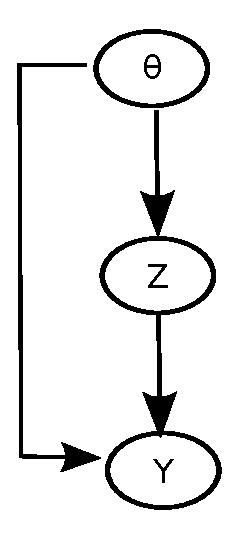
\includegraphics[scale=0.5]{ModHier.pdf}
\end{column}
\begin{column}{0.8\textwidth}
\paragraph{Bayes Formula}
{\small
\begin{align*}
P(\Ybf, \Zbf;\thetabf) & = P(\Ybf\vert \Zbf; \thetabf) P(\Zbf; \thetabf),\\
& = \textcolor{orange}{P(\Zbf\vert \Ybf; \thetabf) P(\Ybf; \thetabf).}
\end{align*}
Therefore,
\begin{align*}
\log P(\Ybf; \thetabf) & = \log \left \lbrace P(\Ybf, \Zbf;\thetabf) / P(\Zbf\vert \Ybf; \thetabf) \right\rbrace\\
& = \log P(\Ybf, \Zbf;\thetabf) - \log P(\Zbf\vert \Ybf; \thetabf) \\
\end{align*}
For a given $\thetabf_0$, we may compute $P_{\thetabf_0}=P(\Zbf\vert \thetabf_0, \Ybf)$ and
\begin{align*}
\log P(\Ybf; \thetabf) &= \Esp_{\thetabf_0}(\log P(\Ybf, \Zbf;\thetabf)) - \Esp_{\thetabf_0}(\log P(\Zbf\vert \Ybf; \thetabf))\\
  & = Q(\thetabf, \thetabf_0) - H(\thetabf, \thetabf_0)
  \end{align*}}
\end{column}
\end{columns}
\end{frame}


\begin{frame}{More generally - EM algorithm}
\begin{columns}
\begin{column}{0.2\textwidth}
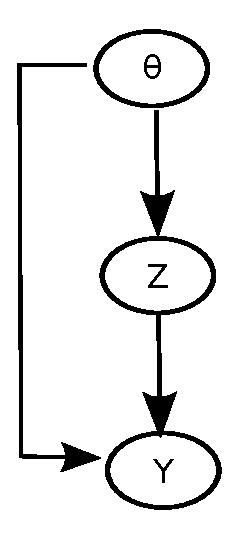
\includegraphics[scale=0.5]{ModHier.pdf}
\end{column}
\begin{column}{0.8\textwidth}
{\small
Since 
$$\log P(\Ybf; \thetabf)  = Q(\thetabf, \thetabf_0) - H(\thetabf, \thetabf_0),$$
and $H(\thetabf, \thetabf_0)$ achieves its maximum in $\thetabf_0$,
\begin{align*}
\log P(\Ybf; \thetabf)- \log P(\Ybf; \thetabf_0)  = & \textcolor{orange}{(Q(\thetabf, \thetabf_0) - Q(\thetabf, \thetabf_0))} +\\&
\textcolor{green}{(H(\thetabf_0, \thetabf_0)-H(\thetabf, \thetabf_0))}.
\end{align*}
}

\paragraph{Expectation - Maximization algorithm}
\begin{enumerate}
\item Phase E : \\
Calculate  $Q(\thetabf,\thetabf^{k})$ for every $\thetabf$.
\item Phase M :\\ Define  
$\thetabf^{k+1}=argmax\, Q(\thetabf,\thetabf^{k})$
\end{enumerate}
\end{column}
\end{columns}
\end{frame}

\begin{frame}{EM algorithm for mixture model}
\begin{align*}
Q(\thetabf,\thetabf^{(\ell)}) & = \Esp_{\thetabf^{(\ell)}}(\log P(\Ybf, \Zbf;\thetabf))\\
    &= \Esp_{\thetabf^{(\ell)}} \left\{\sum_i \sum_k Z_{ik} [\log \pi_k + \log
      f_{\theta_k^{(\ell)}}(Y_i)] \right\}\\
    &= \sum_i \sum_k \Esp_{\thetabf^{(\ell)}](Z_i = k | Y_i) \log\left[\pi_k f_{\theta_k^{(\ell)}}(Y_i)\right]
  \end{align*}
  Recall that $\tau_{ik}^{(\ell)}:=P_{\thetabf^{(\ell)}(Z_i = k | Y_i )$
  \begin{align*}
    Q(\thetabf;\thetabf^{(\ell)})
    &=\sum_i \sum_k \tau_{ik}^{(\ell)} \log \pi_k +  \sum_i \sum_k \tau_{ik}^{(\ell)}\log f_{\theta_k^{(\ell)}}{(Y_i)}\\
  \end{eqnarray*}
  $\rightarrow$ Need to estimate $\tau_{ik}^{(\ell)}$
\end{align*}
\end{frame}
\subsubsection*{Assumptions}
\subsection{Example}
\subsection{Theoretical aspects}
